%-----------------------------------------------------------------------------
%
%               Template for sigplanconf LaTeX Class
%
% Name:         sigplanconf-template.tex
%
% Purpose:      A template for sigplanconf.cls, which is a LaTeX 2e class
%               file for SIGPLAN conference proceedings.
%
% Guide:        Refer to "Author's Guide to the ACM SIGPLAN Class,"
%               sigplanconf-guide.pdf
%
% Author:       Paul C. Anagnostopoulos
%               Windfall Software
%               978 371-2316
%               paul@windfall.com
%
% Created:      15 February 2005
%
%-----------------------------------------------------------------------------


\documentclass{sigplanconf}

% The following \documentclass options may be useful:

% preprint      Remove this option only once the paper is in final form.
% 10pt          To set in 10-point type instead of 9-point.
% 11pt          To set in 11-point type instead of 9-point.
% authoryear    To obtain author/year citation style instead of numeric.

\usepackage{amsmath}
\usepackage[pdftex]{graphicx}    
\usepackage{wrapfig}

%Listings package setup
\usepackage{listings}
\usepackage{color}

\renewcommand{\lstlistingname}{Listing}% Listing -> Algorithm
\renewcommand{\lstlistlistingname}{List of \lstlistingname s}% List of Listings -> List of Algorithms

\definecolor{dkgreen}{rgb}{0,0.6,0}
\definecolor{gray}{rgb}{0.5,0.5,0.5}
\definecolor{mauve}{rgb}{0.58,0,0.82}

\lstset{
  language=Java,
  aboveskip = 3mm,
  belowskip = 3mm,
  breaklines = true
}

\begin{document}

\special{papersize=8.5in,11in}
\setlength{\pdfpageheight}{\paperheight}
\setlength{\pdfpagewidth}{\paperwidth}

\conferenceinfo{CONF 'yy}{Month d--d, 20yy, City, ST, Country} 
\copyrightyear{20yy} 
\copyrightdata{978-1-nnnn-nnnn-n/yy/mm} 
\doi{nnnnnnn.nnnnnnn}

\titlebanner{banner above paper title}        % These are ignored unless
\preprintfooter{short description of paper}   % 'preprint' option specified.

\title{ENGR440 HCI - Final Project Report}
\subtitle{Part One - Project Report}

\authorinfo{Iain Walker}
           {300212708}      


\maketitle

\begin{abstract}

Leap Motion is appearing as a potential technology to bring gesture-controlled systems into the wider consumer market. This report reviews the construction of a Google-Maps like interface for Leap Motion, controlled by gestural input. The system developed which I call 'Leap Earth' is described, and the gesture and interface design decisions analysed. Discussion around the real limitations of current Leap Motion software leads to the argument that current gesture systems are still in a gimmicky phase. However current tooling around the Leap SDKs is extremly well designed, despite the inherent complexity introduced when developing for a 3D interface.

\end{abstract}

\section{Introduction}

Gestural interfaces are an emerging challenge for interface designers, with succesful and extremely fine-grained control mechanisms such as the Leap Motion appearing in the consumer market. Mapping applications are widely used on multiple platforms; interfaces with mapping software have been designed using traditional keyboard/mouse setups, touchscreen and even voice controlled GPS systems - all of which have been successfully adopted in the consumer market. An equivalent prototype using gesture control would be an interesting experiment.

The remainder of this paper is structured as follows. Section \ref{sec:leap_system} looks at the Leap Earth system implemented, as well as a brief description of the technologies used in implementation. Section \ref{sec:design_decisions} analyses user interface design decisions taken whilst implementing the system, with regard to interface layout and supported gestures. Section \ref{sec:leap_interaction} critiques the effectiveness of the Leap Motion for controlling interfaces, whilst Section \ref{sec:leap_development} reviews how useful the Leap SDKs are for constructing quality software.

\section{Leap Earth System}
\label{sec:leap_system}

The Leap Earth System created is intended to be a prototype for a more natural gestural interface for navigating a Google-Earth like application. Navigating current Google or Apple map systems with a mouse and keyboard or touchscreen is relatively straightforward. A more natural gestural interface is an interesting domain when considering applications that are easily grasped already with existing technologies. 

The Leap Earth system simply consists of a map rendered on a globe that may be interacted with using gestures. As we zoom in and out, more or less detail is displayed on the globe. Actual features of mapping software (e.g. consider Google Maps direction function) are out of the scope of this project. Rather the focus of implementation has been experimentation with various gestural control styles of the globe itself. One feature added to demonstrate additional layered interaction was the placing of markers on the map. This was added as part of a prototype of the directions use-case for Google maps; we must firstly place two markers that the mapping software will provide directions between.

% This was added as part of consideration of the directions use-case for Google Maps; we must firstly place two markers that the mapping software will provide directions between. 

\begin{center}
\begin{figure}[h!]
\centering
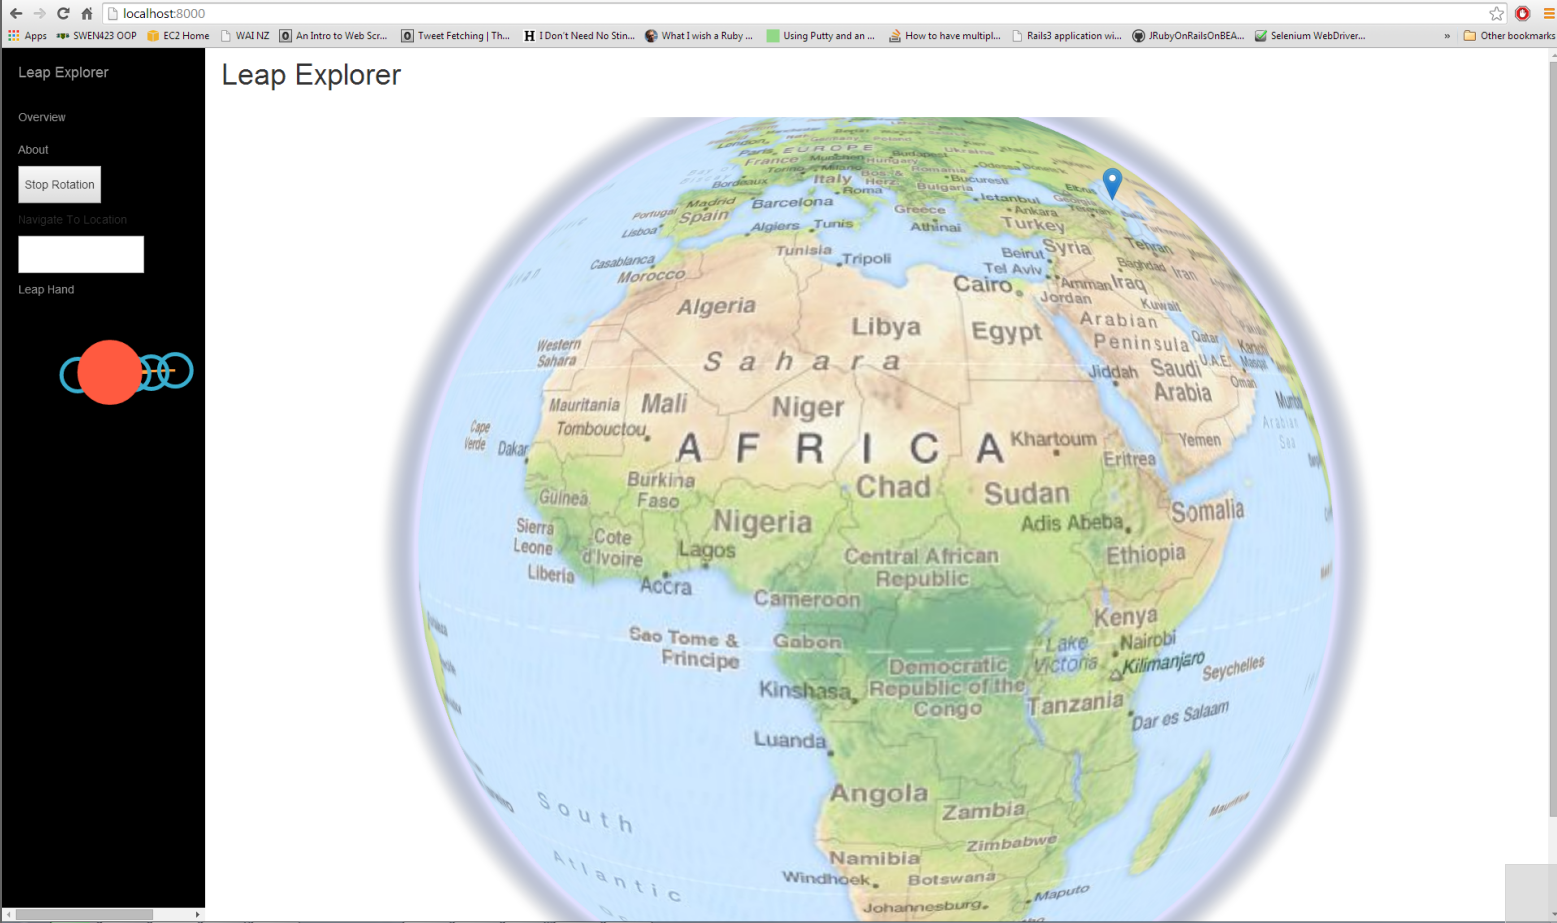
\includegraphics[width=150px]{images/entire_interface.png}
\caption{Entire Leap Earth Interface - globe and sidebar shown}
\label{fig:halo_comparison}
\vspace{-10pt}
\end{figure}
\end{center}

Gestural features supported for globe interaction are primarily based on navigation around the globe. Moving the hand left moves the globe left; moving the hand right moves the globe right, and the same for up and down movements. Zooming is controlled by either moving the hand up or down, or via a finer-grained finger rotation gesture. Finally, perfoming a finger 'flick' action will place a marker at the center of the screen. Arguments supporting the gestural features included are given in Section \ref{sec:design_decisions}.

As well as the primary globe at center screen, a basic side-bar provides some extra functionality. There is a link to an 'about' page, that provides some description as to the purpose of the system, as well as the gestures supported. A stop rotation button allows for pausing of all animations, which was added for debugging purposes early in the project. A 'navigate to location' text box was also placed in the sidebar. This allows the user to type in some location - e.g. 'Wellington', which will cause the globe to rotate and zoom on that particular location. Finally, a Leap Hand is rendered in the sidebar, displaying precisely what the Leap Motion device sees in real time. 

\begin{center}
\begin{figure}[h!]
\centering
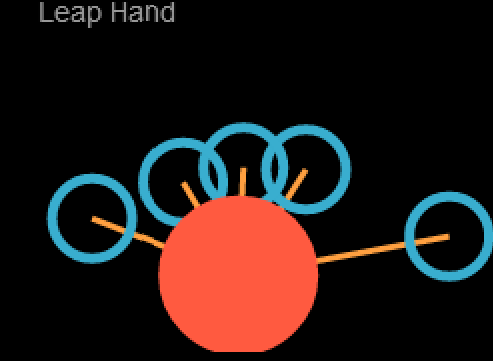
\includegraphics[width=150px]{images/palm_spread_zoom.png}
\caption{Leap Hand from sidebar - displaying palm with spread fingers}
\label{fig:halo_comparison}
\vspace{-10pt}
\end{figure}
\end{center}

\subsection{Implementation Tools}

The Leap Earth system was implemented using the Leap Motion javascript API \cite{leap_js}, running on a basic Python HTTP server. The globe is rendered using the WebGL Earth API \cite{web_gl_api}, and interfaces to tools such as Google Maps API \cite{google_map_js_api} for lookup and coordinate systems. The interface has been tested to work with Google Chrome above version 9 (not currently installed on ECS workstations).

\section{Interface Design Decisions}
\label{sec:design_decisions}

The core design decisions relate to the gestural input design, as the interface layout itself is very straightforward. 

\subsection{Navigation Gestures}

The basis of the navigation gestures provided was built from imagining panning a virtual camera over the global map provided. This camera is held in the palm; thus moving the palm left moves the position shown left; right moves it right, and so on. Initially the approach I wanted to take revolved around holding a virtual soccer ball in two hands, and navigating around the globe as you might inspect or rotate such a virtual sphere in your hand. This proved too innaccurate and difficult to implement. Recognition of the detailed gestures necessary to rotate in such a fashion is not something the Leap Motion is very good at. Immediate detection of gestures is not consistently forthcoming, as will be discussed in more detail in Section \ref{sec:leap_interaction}.

% actual recognition of these quite detailed gestures necessary to rotate such an object is not something that the Leap Motion device is very good at to a high degree - immediate detection of gestures is not consistently forthcoming, as will be discussed in more detail in Section \ref{sec:leap_interaction}.

Having instead deciding on a camera-based approach, actual implementation strategies were considered. Leap Motion examples online actually demonstrate interaction with a Globe, using hand position to control camera position as desired. However these used an approach of directly mapping hand position in the plane detected by Leap Motion into a corresponding globe position and rotation. This is clearly not suitable when considering a mapping tool that must provide navigation capabilities up to very high levels of zoom, as very small movements would correspond to massive distances when implemented on the scale of the globe. Further, removing the hand from the leap motion space will reset the globe's position in these examples. Instead the relative magnitude of hand translation between frames corresponds to movement of the globe, as shown in the formula below.

\begin{lstlisting}
 var newLng = lng +  Math.sin(rotateX * Math.PI/180) * getSensitivity(earth); //sensitivity changes based on current zoom level
\end{lstlisting}


The actual mapping from size of hand movement to amount of rotation induced relates to the current level of zoom, as demonstrated in the formula. This currently followed a simple 50/currentzoom squared formula, which was simply worked out through trial and error. This mapping from zoom to magnitude of translation is not perfect, as small movements at high levels of zoom still have quite large results in camera movement. With a better mathematical understanding of zoom levels to magnitude of movement required though, this could be improved. 

\subsection{Finer Zoom Control}

The challenge of mapping small hand movements onto a surface as large as the globe affected implementation of zoom adjustment also. The Leap zone of detection was simply not large enough to only implement zoom related to how high the hand is held. As such, a circling finger gesture was added to facilitate finer grained zoom control. Circling the finger clockwise increases zoom, whilst anti-clockwise movement decreases zoom. This was simply based off intuition - 'lefty loosey righty tighty'. One of the challenges of course with adding further gestures to a system that implements globe rotation based off of hand position is that the Leap Motion regularly interprets the circling finger as the palm actually changing position. As a countermeasure, during detection of a current finger-circling gesture, any movement of the hand itself is ignored. This interpretation of gestures as hand movement was a difficulty with every single additional feature I attempted to add to the system - which we will review in Section \ref{sec:leap_interaction}.

A potential future solution to this issue of false-positive palm movement could be to implement a 'dead zone' of slight movements, which are just thrown away. In a basic sense I experimented with this - naiively completely ignoring any movements around 0.1 'Leap Units'. The problem with this approach was that it was still not enough to get rid of movement when circling the finger. Further, any larger dead zones made navigation around the world rather unintuitive, as small movements would result in no change, but when the dead zone boundary was breached a sudden large judder would result. This was detrimental enough that I considered the screen locking approach the best one for the prototype at least.

\subsection{Placing of Markers}

The final action possible on the main earth section is the placing of coordinate markers. This was considered as part of a possible wider future use case, in which users place markers and then for example request directions between the two markers. It was also a relevant way of investigating the very real problem of layering additional features onto a gestural system. The gesture to place coordinates is what Leap Motion calls a 'ScreenTapGesture' - a forward tapping movement by the finger. This seemed the most natural way of placing markers on a map as currently supported by the existing Javascript gesture API. 

It is likely that at this stage the reader is thinking of the circling gestures, and how false palm movement detection resulted in undesired globe rotation. The output for a jerky finger tap is, as one would expect, even worse. Again, implementation of a dead zone could have helped with this, but at such a detriment to overall usability that this was considered infeasible. Other gestures were again considered. Certain hand positions (e.g. ball the fist) could have corresponded to placing the coordinate, or any other number of hand poses not requiring actual hand movement. However I considered part of the goal of the system to look at how natural and intuitive interaction styles would work - and really there was no sensible mapping from hand poses into marker placement. Further, what part of the pose constitutes actual placement - when one enters the pose, or exits the pose? These considerations made me prefer the flawed, but ultimately more natural finger tap gesture.

\begin{center}
\begin{figure}[h!]
\centering
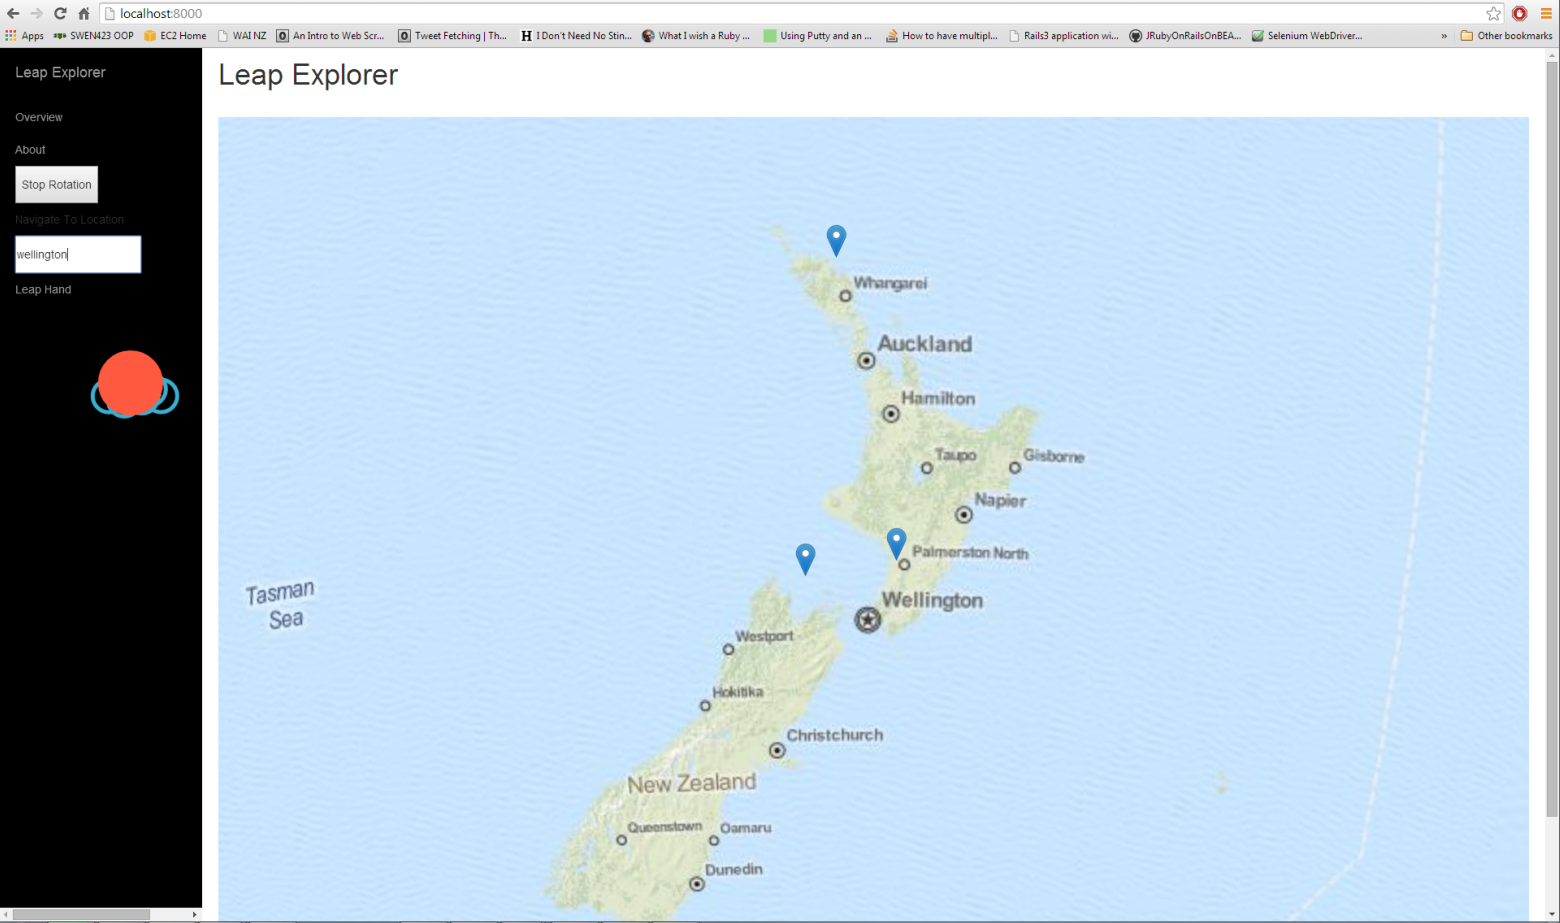
\includegraphics[width=150px]{images/marker_placement.png}
\caption{Placement of markers - difficulty of maintaining accurate placement is fairly apparent}
\label{fig:halo_comparison}
\vspace{-10pt}
\end{figure}
\end{center}

\subsection{Sidebar Design Decisions}

The Sidebar design was inspired by the overall layout of Google Maps, which has the simple UI of the map itself and a bar with relevant informative messages etc to the left of the page. 

The only feature significant enough for discussion on the sidebar is the Leap Hand box, which renders a view of what the Leap Motion device sees in real time. This was originally implemented as a learning exercise and to debug Leap Motion gestures and hand positioning. Having the Leap Visualiser and my site open on a single-monitor workstation was proving impractical, and thus immediate feedback of what the device was detecting was useful for development purposes. However having shown the website to friends, I receieved comments that having the Hand shown helped with learning the mechanics of the Leap technology. Issues such as where the Leap detects, whether the Leap is detecting my hand(s) currently, and any potential occlusion are immediately highlighted by the Leap Hand box, which still manages to take up very little screen real estate. 

\subsection{Further Discarded Gestures}

There were a few gestures I implemented that were ultimately discarded for a number of reasons. I intended to add a 'swiping' gesture, that would result in the earth rotating at a set speed in the direction of the swipe. Further swipes in the same direction would increase the speed of rotation, as with spinning a basketball on your finger for example. Implementing such a gesture unfortunately again clashed with the positional manipulation of the globe. Swiping was actually completed before the positional mapping was working correctly, but having added the positional control the side-effects of swiping were too greatly pronounced for the feature to remain.

We can see that further gestures clashing with existing ones, as well as gestures in general clashing with positional control as being a recurring theme in my project. As an inexperienced developer of gesture controlled interfaces, this was unfortunately something I did not anticipate. If I was to develop further interfaces with the Leap Motion device, I would certainly consider carefully what gestures could be implemented in tandum for the problem domain, as well as considering in advance whether the gestures would cause conflicts. With the technology at hand, simple interfaces with a small range of possible interactions may be the best for gesture based systems. Although the Leap Earth system is very basic, there was still room for gesture conflicts to occur, particularly with the positional control employed.

Having reviewed the Leap Earth system developed, and discussed core design decisions relating to the interface and gesture interaction, we will now look at the Leap Motion controller as an interaction device.


\section{Leap Motion Interaction} 
\label{sec:leap_interaction}

\subsection{Consumer Focus}

As a peripheral device for a computer, the Leap Motion is as easy to install and setup as one would expect it to be. Every system I have plugged the Leap Motion into detects the controller immediately and installs the relevant packages required to get the software running. The fact that a Leap Motion focused application store comes packaged with the basic software downloads increases the ease of learning how to control with the system. With a multitude of basic games at your fingertips, getting started is a breeze. The Leap device itself is also extremely unobtrusive. One does not notice it taking up any room on your desk. The technology behind the Leap Motion is also basic enough that the device is affordable to consumers. It uses infrared optics and cameras instead of the Kinects depth sensors, at much higher fidelity than the Kinect, at a refresh rate higher than computer monitors \cite{}. The software backing the device is what really sets it apart, though; algorithms for which are being (understandably) kept very secret. Thus from a consumer perspective the Leap Motion has taken the right approach. 

\subsection{Accuracy Issues}

It was after getting started, and the exciting novelty of controlling applications with my hands wore off that real issues with the accuracy of the device became more noticeable. Whilst the fidelity of the device is extremely high, when experimenting with the visualiser you can see how often fingers cut out or fuse together. Detection of hands themselves sometimes fails, with a hand disapearing for a second. 

Occlusion is of course an issue, and where one hand or parts of a hand block fingers (for example when a hand is turned sideways) the Leap Motion has real difficulty detecting what is going on. This results in some unexpected hand models. Occlusion is potentially solveable using two Leap Motions however, as discussed in class.

A constant problem with the Leap Motion is getting a feel for the boundaries of the device. In most applications there is no supported reference for whether your hands are within the bounding box of detection area. I attempted to address this in my application, but the immediate and sudden loss of control is still an issue. There appears to be no blurred edge to the Leap boundary; you are either detected or not. Perhaps this was a design decision to immediately cut off the hand rather than attempt to poorly model hands when they approach the edge of detection area. Online critiques of the Leap Motion support this claim; in action games for example, hands would often come outside the bounding box in writers' excitement, resulting in immediate loss of control \cite{leap_review}. 

\subsection{Difficulty Detecting Gestures}

The innacuracies of the Leap Motion detecting hand position and posture are mild in comparison to Gesture recognition however. The main problem I faced when implementing a swipe gesture originally for the Leap Earth was actually figuring out how to perform a swipe that the Leap device would detect consistently. It seems like gestures have to be performed in a very rigorous, well-defined manner for the Leap Motion to recognise the action as a supported gesture. It is worth noting that my difficulties in figuring out a reproducable swipe action were encountered after reading developer documentation for what constitutes a swipe action - this would likely be more unintuitive for a casual user coming to the device. The exagerated gesture needed to register a swipe was part of the reason I had to remove it from the Leap Earth application - if a subtle swipe was enough to register, it may have been maintainable.

\subsection{User Fatigue}

Something that rarely occurs with the traditional mouse and keyboard setup is user fatigue. However with the Leap Motion, after holding my hands in the air for extended periods of time I found myself getting tired. Despite the tag of natural and intuitive interaction given to Leap Motion, it is actually not particularly natural to sit with arms extended for long periods of time. This was mitigatable at my desk my resting my elbows on the seat armrests, but was still a much more effort-inducing posture than typing on a keyboard. I wonder how Occupational overuse syndrome (OOS) would fare with long-term uses of the Leap Motion - surely the requirement for significantly more muscle use than the keyboard/mouse, and little more oxygen moving through the body would be a prime cause of OOS.

\subsection{Device Unresponsiveness}

One unusual and recurring issue with the motion device is that it would frequently become unresponsive, with the only way to get it started again being to unplug it and plug it back in again. This would generally occur after a period of unuse, but also occasionally occured during interactions. It was not immediately obvious that the device had stopped detecting input, as in the Leap control panel it was still claiming to be active. I am not sure if this is a defect with the particular model I have, or a more general issue, as I could not find evidence of others experiencing the same difficulties online.

\subsection{New Design Considerations}

Following discussion in class about designing for intuitive gesture based interfaces, I imagined that implementing an interface based off pure gesture recognition and interaction would be relatively straightforward. However the difficulty with the device recognising hand position and gestures made this task more complicated than I envisaged. The lack of established standards and rules also means that experimentation is the rule of the day; it is still difficult to predict whether a set of gestures will work together and not conflict. 

The above difficulties with both designing interfaces for Leap Motion and actually using the tool accurately mean that I believe the Leap Motion is still at a gimmicky stage of gesture-based interface design and use. While the tool was fun to play with and build a tool for, at this stage the real limitations with its use mean I could not envisage it as a serious industrial tool. 

\section{Leap Motion Development}
\label{sec:leap_development}

The Leap Motion was a nice tool to develop software for, reasons for which will be discussed now.

\subsection{Getting Developers Started}

A goal for the creators of Leap Motion is surely to get as many developers working with the software as possible. The approaches taken by Leap Motion has strongly supported this aim. A common starting point for developers when learning a new tool is to want to dive into some code and get a feel for the system. There are very detailed tutorial examples online for Leap Motion. Step-by-step instruction is provided to the software design of the Leap Controller, into rendering what the Controller sees, into adding suported gesture recognition and response. If these tutorials are not enough, many developers have posted code online demonstrating their own basic Leap Motion applications, which is of further benefit when moving through the learning process of understanding a new tool. 

The multitude of supported languages for developing with Leap is of great advantage also. Javascript, C\# (with Unity support), C++, Java, Python and Objective-C are all supported, which in the current code climate is enough to represent languages for basically every platform available. Leap Motion developers are in no means limited by choice of API or platform.

\subsection{Programming Model}

The only API I worked with was the Javascript API, largely because working with Javascript and HTML is a very straightforward means to getting a basic interface up and running quickly (e.g. compared to Java Swing). The Leap Motion programming model whilst working with the Javascript API is very sensible, basically just consisting of a single programming loop, following reactive programming models. This works well with web documents, as the loop refresh is about as fast as page refresh. This allows for very smooth manipulation of objects, as seen with the Leap Earth system - manipulation of the globe is very smooth. Incorporating the Leap API into a javascript application is extremely straightforward - a single import to an online document means the API can be updated without programmer effort to download the latest version and incorporate it into an application. This means we have to trust the Leap Motion devs not to break our code during updates of the API - hopefully a reasonable assumption. 

The model for detecting position and movement is extremely powerful - it allows for comparison between previous frames and distance vectors on every element detected by the Leap Motion device. Multiple previous frames are stored, allowing for flexible comparisons dating back to the past few seconds. 

Despite the limitations of accuracy, the gesture model is also fairly powerful and easy to use. Within the main controller loop, the gesture detection can be added simply by referencing the current frame and asking for any gestures contained in the frame. Gesture type may then be queried, and reaction to gesture coded accordingly. Whether the gesture has just started, is ongoing, or has finished is also easily accesible - important information for potentially lengthy gestures such as swipes. User defined gestures can also be created as Objects within javascript code, and then queried as per standard gestures defined in the Leap API. 

\subsection{3D Interfaces and Mathematics}

One of the difficulties I encountered developing for the Leap Motion was not caused by the Leap APIs themselves but by the very nature of programming for a 3D interface. There is more maths involved when converting a 3D model into a essentially 2D interface. This style of coding would possibly be more familiar to programmers who have experience with graphics programming for example. Seeing examples online littered with sin and cosine functions was the most daunting element of learning Leap Motion. This was also a element of designing a system responding to changes in 3D vectors - simply making an interface respond to chosen gestures is a more straightforward challenge, despite the limitations of Leap Motion gesture detection.

\subsection{Lack of Standards}

Again the lack of standards within the current gestural-interface community is an interesting challenge when developing with the Leap Motion. I am conflicted as to whether this is a good or bad thing for developers - it is possibly too early in gestural interface development to implement defined standards, at the risk of killing creativity. However as someone who personally likes to extend off example rather than experiment with totally new features, I would have liked some more example programming style and gestural design information to base my application off.

\section{Conclusion}

The Leap Motion is a new and exciting gesture recognition device, that has resulted in fairly high use by developers. My project to experiment with the Leap Motion kit was a Leap-Earth interface, intended to be similar to a 3D Google-Maps interface controlled soley by gestures. This was a sucess, despite difficulties around conflicting gestures which are possibly a wider symptom of issues with 3D interfaces currently. Unfortunately such innacuracies may render the Leap Motion as a gimmicky interaction mechanism, but it certainly presents a range of opportunities for future gestural interface development. Developing with the Leap Motion was straightforward to learn given the added complexity of a 3D interface, however the issues around gestural detection and accuracy of detection mean that very basic interfaces are all that may be controlled by this device at present. 

%Having had little experience with graphics programming 

% These include links to an 'about' page which describes the supported gestures, a 'stop' button (which cancels all movement on page), a na

% Gestural features supported include the navigation around the globe; panning left, panning right, up and down. Zoom is supported through hand movement and a finer-grained finger rotation gesture. 

% Gestural design is based upon imagining controlling a camera that rotates around the virtual sphere - or in this case the globe rendered in the main view. 


% The actual gestural design was initially based upon imagining how I would interact with a virtual spherical object. 



% The Leap Earth System was intended to be a more intuitive interface for navigating a Google-Earth like environment. Whilst navigating current Google or Apple map systems with a mouse and keyboard setup is fairly straightforward, a more natural intuitive gesture controlled system would be an interesting experiment. The Leap Earth system constructed simply consists of a globe which may be rotated and interacted with as one would rotate a football-like sphere in an invisible plane. For example, moving the hand left moves the globe left, moving the hand forward moves the globe up, and moving the hand up or down controls the zoom level of the map. Responsiveness of the various movements is relative to how far zoomed in the camera is - for example at low levels of zoom, rotating the entire globe is possible, whereas at higher levels finer grained control is required. 



% The interface consists only of the main Globe and a side-bar to assist navigation and provide links to an 'about' page. On the side bar, a 'leap hand' image is provided which renders the hands that the device currently sees. I initially built this for debugging and learning purposes, but left it in the application following feedback that it provided useful context about what the sensor device could see. 

%TODO insert image of the hand visualiser

% The main globe is where exploration of the globe can occur. This was built using the WebGL Earth API, which provides an inbuilt-globe rendering to an HTML page with a javascript API for performing operations on the globe. A full description of the features of the API is available at \cite{}.

% The Leap Earth system is a globe rendered on an HTML page, which I have running on a Python HTTP server. 

% As such, one aim of this prototype was to investigate how gestural interfaces could perform in an application domain where the equivalent standardised interactions are easily grasped.


% \subsection{Gesture Design}




% \section{Interface Design Decisions}








%\subtitle{Part Two - Experiment Report}

% By demonstrating largely through example how modularity and concurrency implementations can be synergystic, a strong argument applying GOF patterns to enhance modularity coupled with an automated concurrent framework were applied to real-world applications. 

% Discussion of the core contribution of the paper being the framework provided. Discuss how its current primary limitation is that it cannot completely abstract parallel programming in every case. In order for this to occur, a complete backend system would need to be developed, rather than the lightweight pattern based system that was implemented.

% \cite{wirfs1989object}

% We recommend abbrvnat bibliography style.

% \bibliographystyle{acm}
\bibliographystyle{abbrvnat}
\bibliography{bibliography}  % often included from a separate file.


\end{document}

%                       Revision History
%                       -------- -------
%  Date         Person  Ver.    Change
%  ----         ------  ----    ------

%  2013.06.29   TU      0.1--4  comments on permission/copyright notices

